\chapter{Particle Reconstruction and Identification}
\label{ch:part_reco}

With a design luminosity of $1.0 \times 10^{34}$ cm\textsuperscript{-2}s\textsuperscript{-1}, and a peak Run 2 instantaneous luminosity of $2.0 \times 10^{34}$ cm\textsuperscript{-2}s\textsuperscript{-1}, reconstructing and identifying the products of LHC $pp$ collisions is one of the most complex tasks for the ATLAS detector. The accurate reconstruction and identification of \textit{physics objects}\footnote{A physics object is a particle or group of particles which has appeared in the ATLAS detector and whose properties have been estimated via the measurements left in various detector subsystems.} lays the ground work for all subsequent physics analyses, so it is also one of the most fundamentally important tasks performed by an experiment. \par

Reconstruction is the process of combining raw and uncalibrated hits across various subsystems into unique objects. Two particular subsystems, the Inner Detector (ID) tracker and the calorimeters play particularly important roles and will be discussed in detail. Analysis of the properties of the reconstructed objects identifies them as photon, electrons, muons, or jets. While photons, electrons, and muons are fundamental particles, jets represent a collimated shower of many hadronic particles, whose definition is more flexible. Jet reconstruction, clustering and track association are all of particular import to jet identification, and to the later content of this thesis. Finally, reconstruction also identifies \textit{missing transverse energy} \met~in events, which is a crucial variable for BSM physics searches. Figure \ref{fig:detector_objects} shows how the physics objects listed here interact with various systems in the ATLAS detector. 

\begin{figure}
        \centering
	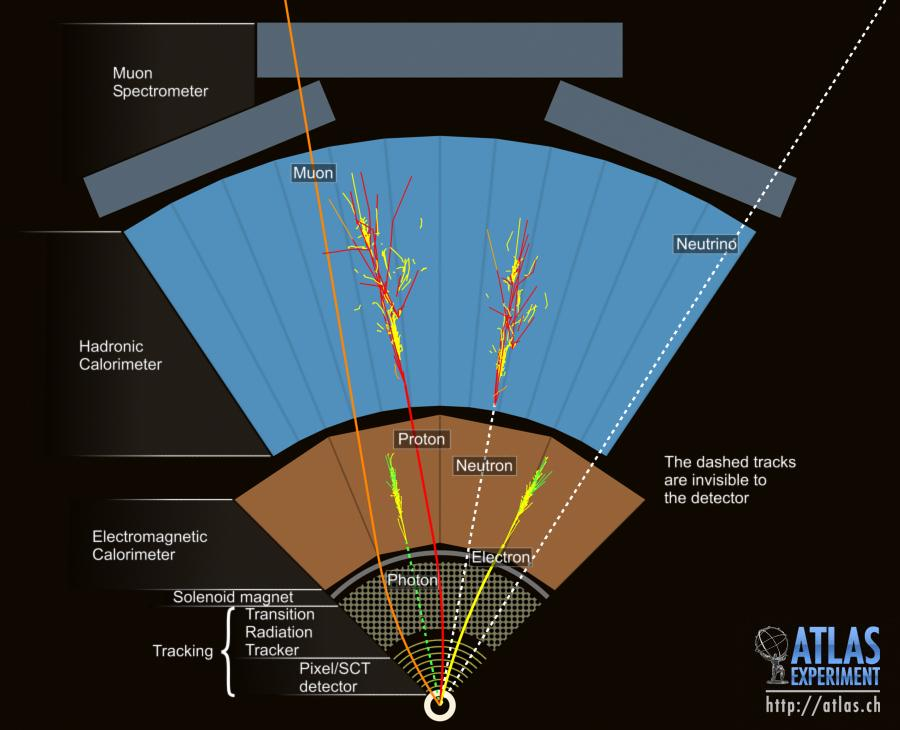
\includegraphics[width=0.7\textwidth]{figures/ch5/detector_objects}
	\caption{This graphic illustrates a slice of ATLAS detector barrel \cite{detector_events}. A photon, electron, and two jets (associated to the proton and neutron) are shown, illustrating each object's interaction with various ATLAS subsystems. The path of the charged particles is curved on account of the strong magnetic field produced by the solenoid and toroid magnets. A neutrino, generally representing the reconstruction of missing transverse energy \met, is also illustrated.}
	\label{fig:detector_objects}
\end{figure}

\section{Inner Detector Tracks}
\label{sec:inner_det_tracks}
As the inner most layer of the detector, the ID measures charged particles close to the interaction point. The various hits of these charged particles throughout the ID are used to reconstruct \textit{tracks} which give the trajectories of charged particles \cite{track_finding}. Track reconstruction begins by clustering hits in the Pixel and SCT detectors, and combining clusters from different radial layers of these detectors. The multi-layer clusters form track \textit{seeds}, which provide initial estimates of measurements belonging to an individual track. The requirement of three points allows for a rough estimate of the track \pt~to be made by calculating the curvature of the track and accounting of the magnetic field in the ID. \par

Track seeds are subject to a variety of quality requirements, such as having a minimum estimated \pt~and passing interaction region compatibility criterion. If these requirements are satisfied, the track seeds are passed to the track finding and fitting algorithms. The interplay of these three track reconstruction steps is illustrated in Figure \ref{fig:track_reco}. 

\begin{figure}
        \centering
	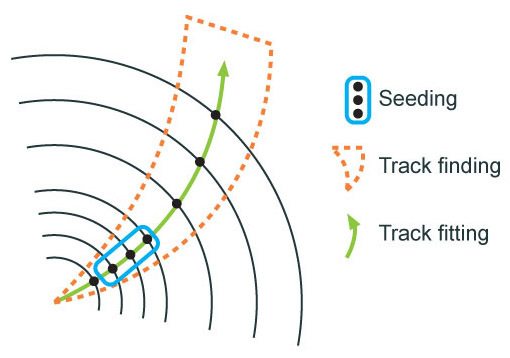
\includegraphics[width=0.6\textwidth]{figures/ch5/track_reco}
	\caption{Track reconstruction seeding, finding and fitting illustration \cite{track_finding}}
	\label{fig:track_reco}
\end{figure}

\section{Photons and Electrons}
Photons and electrons shower in the LAr calorimeter, and are identified by the energy deposits they leave there. Energy deposits in a collection of nearby cells are termed \textit{proto-clusters}, which become the starting point for electron and photon reconstruction \cite{electron_photon}. The clustering algorithm begins when the energy deposit in a certain cell exceeds the noise threshold with a significance of 4$\sigma$. The algorithm then collects neighboring cells which have an energy deposit exceeding the noise threshold with a significance of 2$\sigma$, creating a \textit{topo-cluster}\footnote{A topo-cluser is a topological grouping of neighboring calorimeter cells based on their energy deposits}. Next, these topo-clusters are matched to ID tracks, created as described in Section \ref{sec:inner_det_tracks}. The location of the topo-cluster defines a region of interest (ROI) in the ID, where additional modified track reconstruction algorithms are run in the case that no associated tracks are found. Any ID tracks associated to the topo-cluster are retrofit to allow for additional energy loss due to bremsstrahlung. A converted photon track reconstruction algorithm is run to check for tracks coming from secondary vertices consistent with converted photons. The secondary vertices are constructed from two oppositely charged tracks consistent with a massless particle, or from one track without any hits in the innermost layer of the ID. \par

For electron identification, the EM cluster is required to match ID tracks that originate from the primary vertex at the interaction point. For photon identification, the EM cluster can either be matched to tracks coming from a secondary vertex (converted photon), or matched to no tracks (unconverted photon). Figure \ref{fig:electron_photon_id} illustrates these three cases for EM object identification. \par

\begin{figure}
        \centering
	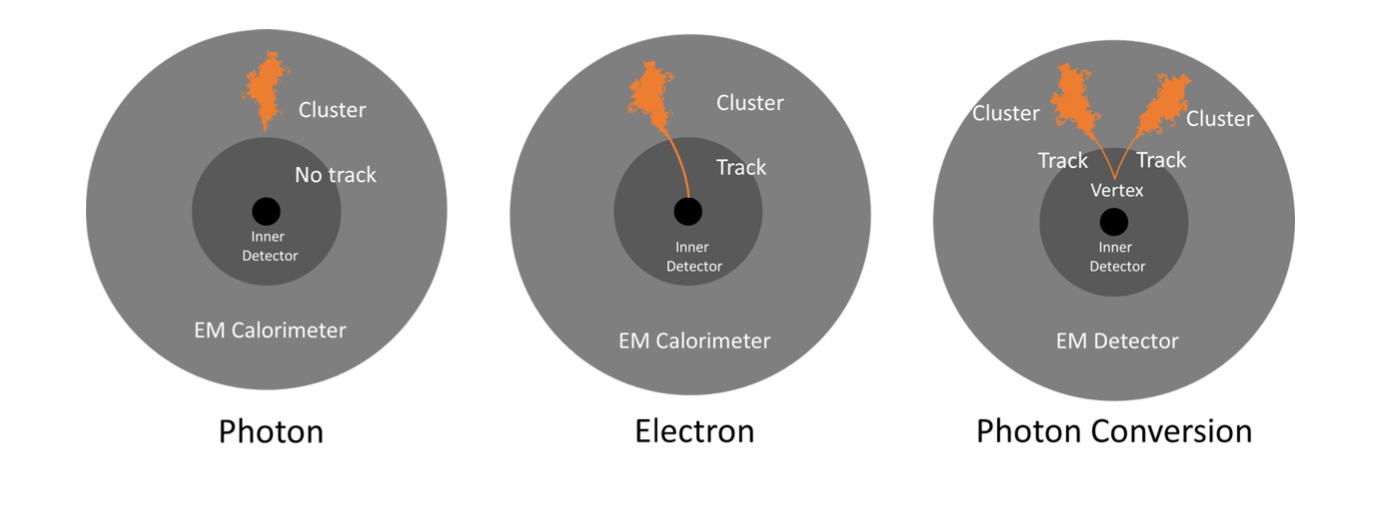
\includegraphics[width=0.9\textwidth]{figures/ch5/electron_photon_id}
	\caption{Three types of EM object candidates \cite{electron_photon_id}. }
	\label{fig:electron_photon_id}
\end{figure}

\textit{Superclusters} are built separately for photons and electrons, based on the combined topo-cluster and ID track information. First, the EM topo-clusters are tested to see if they meet the minimum requirements to become electron or photon seed clusters. For electrons, the cluster must have a minimum \et~of 1 GeV, and must be matched to a track with at least 4 hits in the silicon tracking detectors. For photons, the cluster must have an \et~greater than 1.5 GeV. If the seed cluster requirements are met, the algorithm searches for satellite clusters, which can arise from bremsstrahlung radiation. If the satellite clusters pass the positional, energy and tracking requirements to be associated with the proto-cluster, they are combined into a supercluster. \par

Electron and photon objects are identified from the superclusters after the energy calibration is applied, which accounts for the energy resolution of each subdetector measurement. Because photon and electron superclusters are built independently, some clusters can produce both a photon and an electron. In this case an ambiguity resolution procedure is applied to determine if the supercluster can be easily identified as only a photon (no tracks present) or only an electron (good tracks pointing to the primary vertex). In some cases, the identity of the cluster is still ambiguous, in which case both a photon and electron object are created for analysis and flagged as ambiguous. Energy, shower shape, and other analysis variables are calculated from the supercluster and saved with the electron or photon object. 

\section{Muons}
Muons are identified through the tracks and energy deposits they leave in the ID, calorimeters, and Muon Spectrometer (MS). Muons experience minimum ionizing loss, meaning the do not deposit much of their energy in the calorimeters (recall Figure~\ref{fig:detector_objects}), and therefore reach the outer regions of the detector where the MS is housed. Muon identification begins in the Muon Drift Tube chambers by performing a straight line fit between the hits found in each layer, creating \textit{segments}. Segments in the middle layers are then used as seeds for the track building algorithm, which searches for compatible combinations of segments based on their relative positions and angles \cite{muon_reco}. A $\chi^2$ fit is performed on each track candidate. Based on the $\chi^2$ criteria, hits are removed or added such that the track contains as many hits as possible while satisfying the fit criteria. \par

The MS track candidates are combined with track information from the ID and calorimeters according to various algorithms based on the information available from each subdetector. Four different types of muons arise from the various reconstruction algorithms: 
\begin{itemize}
  \item Combined muon: a muon track identified through independent track reconstruction in the ID and MS, where the combined track is formed using a global refit that uses hit information from both detectors. Most muons are constructed through an outside-in procedure, in which a muon track candidate is identified in the MS and then an associated track is found in the ID. A complementary inside-out procedure is also implemented and identifies additional muons.
  \item Segment-tagged muon: an ID track is identified as a muon if when extrapolated out to the MS (following the inside-out global fit procedure) it is matched to at least one local MS segment. 
  \item Calorimeter-tagged muon: an ID track is identified as a muon if it is matched to a calorimeter energy deposit that is compatible with a minimum-ionizing particle. This muon identification has the lowest purity, but it used in regions where the MS has only partial coverage due to cabling and service access routes.
  \item Extrapolated muons:  the muon is reconstruction only from the MS track and a requirement on compatibility with the primary interaction point. The muon track is required to cross at least two layers of the MS, and three layers in the forward region. These muons are mainly used to extend muon acceptance into the region 2.5 < $|\eta|$ < 2.7 where ID track information is not available.
\end{itemize}

Figure \ref{fig:muon_tracks} illustrates the four types of muon reconstruction. Overlap between reconstructed muons using ID tracks is resolved by giving preference to combined muons, then segment tagged muons, and finally calorimeter tagged muons. Overlap with extrapolated muons is resolved by giving preference to the muon with a better fit quality and higher number of tracks. \par

All muon track candidates are required to pass a series of quality selections to be identified in the final muon collection. The primary qualities considered are the $\chi^2$ goodness of fit for the global track, the difference in \pt~measurement between the ID and MS tracks, and the ratio between the charge and momentum of the tracks. The quality requirements help reject hadrons, primarily from kaon and pion decays. Muons candidates consistent with cosmic rays are also rejected.

\begin{figure}[h]
        \centering
	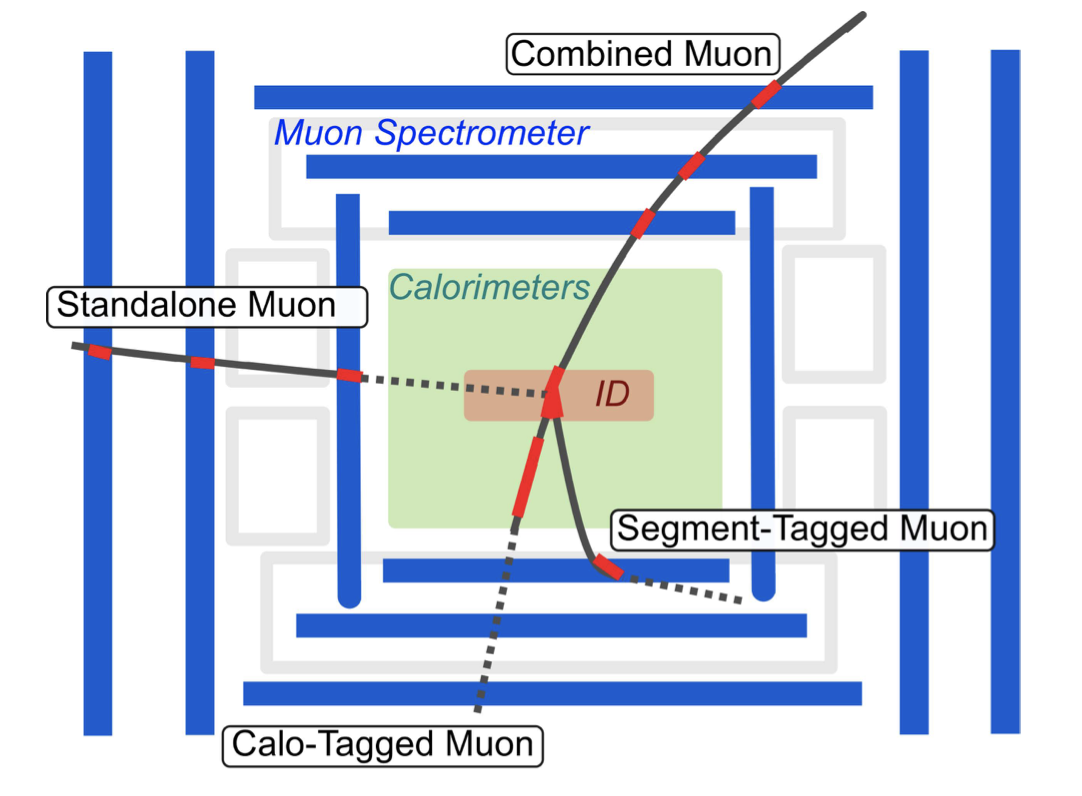
\includegraphics[width=0.6\textwidth]{figures/ch5/muon_tracks}
	\caption{The four types of muon track candidates \cite{muon_id}. The red bands indicate where detector measurements for each much track candidate are made. The dashed lines indicate the path of the muon through detectors where no measurement is made. Standalone muon is another term for an extrapolated muon.}
	\label{fig:muon_tracks}
\end{figure}

\section{Jets}
The protons accelerated in the LHC are composed of quarks and gluons, and thus their collisions often result in the release of energetic quarks and gluons, collectively termed \textit{partons}. The energetic partons can radiate additional gluons, and these gluons can pair produce quarks in a process called \textit{fragmentation}. Fragmentation continues until the energy drops sufficiently that color conservation plays a dominant role. At that point, additional quarks and gluons are produced from vacuum to create neutral color states for the fragmented collection of partons. This process is known as \textit{hadronization} \cite{fragmentation}. The hadronized partons compose a collimated stream of particles, known as a \textit{jet}, which is then observed in the detector. The full process that produces jets is known as a \textit{parton shower}, and is illustrated in Figure~\ref{fig:parton_shower}. 

\begin{figure}[h]
        \centering
	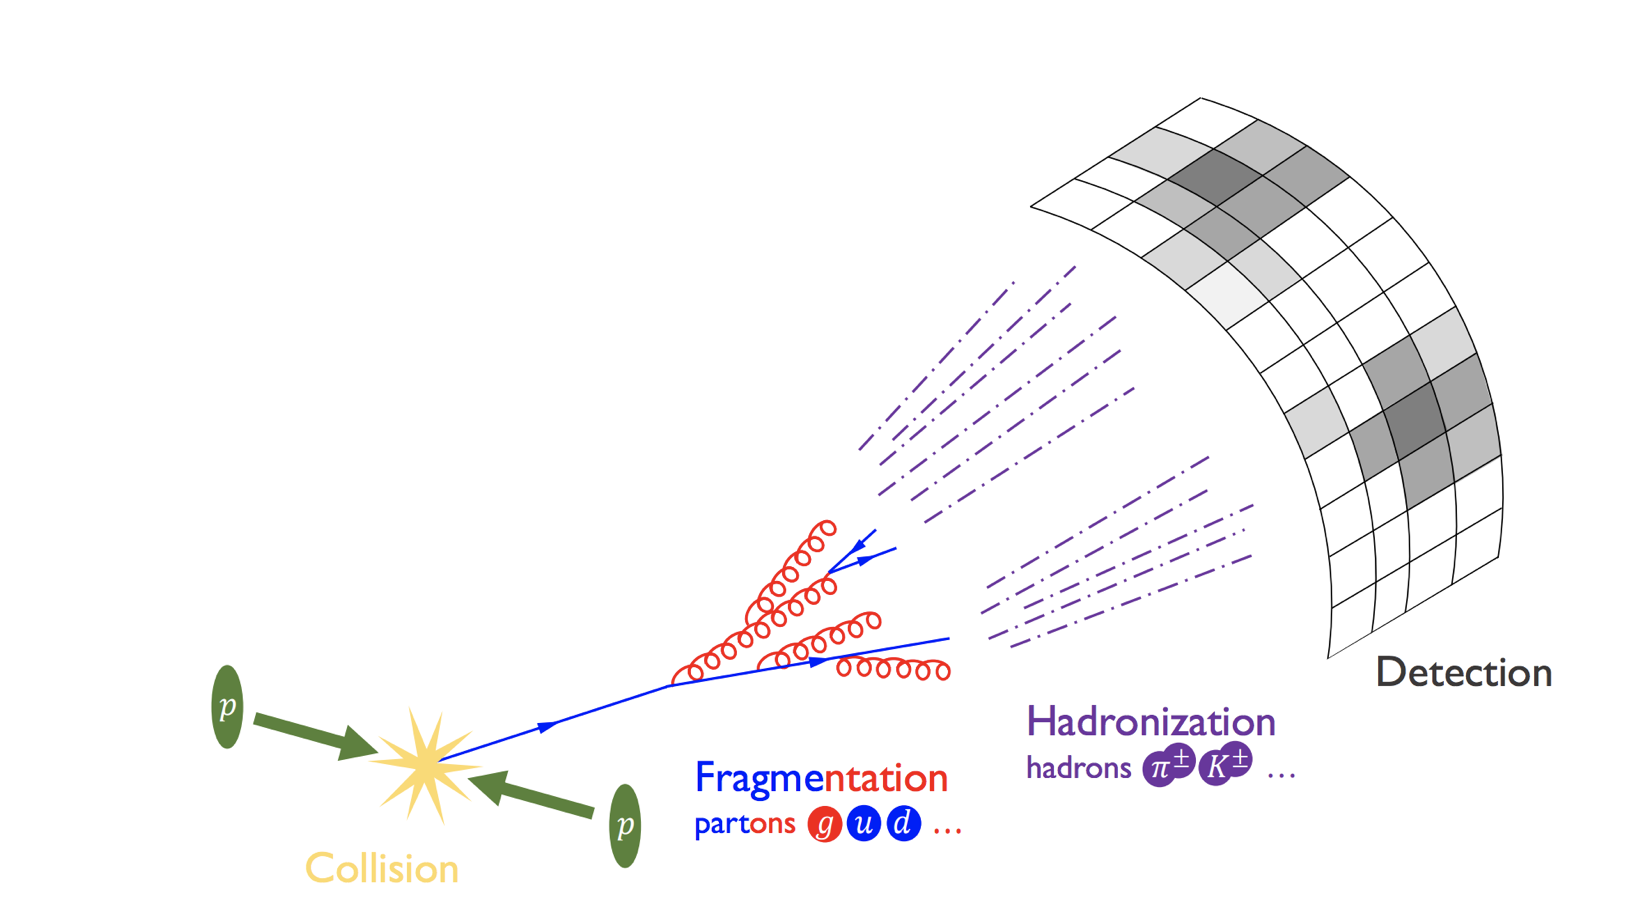
\includegraphics[width=0.75\textwidth]{figures/ch5/parton_shower}
	\caption{The fragmentation and hadronization processes undergone by a quark produced in a proton-proton collision \cite{frag_im}. }
	\label{fig:parton_shower}
\end{figure}

Jets are identified by the energy deposits they leave in the calorimeter, which are then matched to the tracks they leave in the ID. Jet reconstruction generally begins in the calorimeters, with the identification of \textit{topo-clusters}. Then jet reconstruction algorithms combine calorimeter information with tracking information. There are a variety of jet collections depending on the exact usage of calorimeter and tracking information in the reconstruction. Some common collections include particle flow jets (PFlow), track calo-cluster jets (TCC), EM topo-cluster jets (EMTopo), and unified flow object jets (UFO). Only particle flow jets will be discussed in greater detail due to their importance in this analysis. The following sections discuss jet identification in the calorimeters, particle flow jet construction using the \textit{anti-$k_t$ algorithm}, jet clustering and jet substructure characteristics.

\subsection{Calorimeter Clusters}
Jets are first identified by the energy deposits they leave in the calorimeters. As for photons and electrons, the reconstruction of jets in ATLAS begins with the construction of topo-clusters, which are topologically-grouped noise-suppressed clusters of calorimeter cells \cite{jet_reco}. The topo-cluster seed is a cell with an energy that exceeds the noise threshold for the cell with a significance of at least 4$\sigma$. Any cells adjacent to the seed cell in three dimensions are added to the cluster if they have an energy deposit of at least $2\sigma$. This process is repeated, growing the cluster, until no adjacent cells exceeding the energy deposit threshold remain. As a final step, all adjacent cells are added to the topo-cluster, irrespective of their energy. \par

The construction process for topo-clusters allows for the possibility that several independent signatures are grouped into one topo-cluster. To correct for this, the topo-cluster is scanned for local maxima, defined by any cell with energy > 500 MeV, and no neighboring cells with greater energy. If more than one local maximum is identified, the topo-cluster is split among the corresponding energy peaks \cite{topo_clusters}. In the event that one cell neighbors two or more local maxima, the cell is assigned to the two highest-energy clusters that it neighbors. This means each cell is shared at most once, between at most two post-splitting topo-clusters.\par

Two measurements for the total energy of the topo-cluster are considered. The raw, or electromagnetic (EM), scale simply considers the sum of energy from all cells in the topo-cluster. The local cell weighting (LCW) scale first classifies clusters as electromagnetic or hadronic, and then applies appropriate corrections for hadronic interactions in the jet energy calculation \cite{jet_reco}. The corrections are derived from Monte Carlo simulations, and account for the weaker response of ATLAS calorimeters to hadronic interactions (ATLAS calorimeters are \textit{non-compensating}\footnote{The response of ATLAS calorimeters is different for EM showers and hadronic showers, since the calorimeter response to hadronic showers is energy dependent}), and hadronic energy losses due to interactions with dead material \cite{topo_clusters}. \par

\subsection{Particle Flow Algorithm}
The calorimeters provide excellent jet energy resolution for high energy jets. However, the granularity of the hadronic calorimeter is restricted to $0.1 \times 0.1$ in $\eta \times \phi$. Combining the information from the calorimeter with tracking information provides superior angular resolution and energy resolution. The particle flow (PFlow) algorithm is one of a handful of algorithms which can perform this task.\par

An overview of the process is given in Figure~\ref{fig:pflow_diagram}. Tracks from the ID which are selected for the PFlow algorithm are required to have at least 9 hits in the silicon detector, and missing pixel hits in places where a hit would be expected. Additionally, the tracks have \pt~> 0.5 GeV, and $|\eta| < 2.5$. The algorithm then attempts to match these tracks to EM scale calorimeter topo-clusters. This matching is performed using the distance metric 

\begin{equation}
	\Delta R' = \sqrt{\left(\frac{\Delta\phi}{\sigma_\phi}\right)^2 + \left(\frac{\Delta\eta}{\sigma_\eta}\right)^2}
\end{equation}

where $\sigma_\eta$ and $\sigma_\phi$ represent the angular widths of the topo-clusters, and $\Delta\eta$ and $\Delta\phi$ represent the distance between the track (extrapolated to the second layer of the EM calorimeter) and the barycenter of the topo-cluster \cite{pflow}. The topo-cluster closest to the track as measured by $\Delta R'$ is considered matched to the track. If no topo-cluster is found within the cone size of $\Delta R' = 1.64$, it is assumed that particle which left the track did not form a topo-cluster in the calorimeter. \par 

The PFlow algorithm predicts the expected single topo-cluster energy for a given track, based on the track momentum and topo-cluster position. This value is then compared to the observed energy of the topo-cluster, and the probability that the particle energy was deposited in more than one topo-cluster is evaluated. If necessary, the algorithm adds more topo-clusters to the track/topo-cluster system, in order to account of the full shower energy of the track particle. \par

To reduce the impact of double counting the energy of a given particle by including both its tracker and calorimeter energy measurements, the calorimeter energy measurements associated to a given track are subtracted from the total calorimeter measurement. If the expected energy deposited by the particle exceeds the topo-cluster energy, the full topo-cluster is removed. If the expected energy is less than the EM scale energy of all the considered topo-clusters, topo-cluster cells are removed one by one, until the full expected energy deposit of the particle has been removed from the calorimeter information. The resulting set of tracks and topo-clusters represent the event with no double-counting of energy between subdetectors \cite{pflow}. This information is passed to the jet-finding algorithm.

\begin{figure}[h]
        \centering
	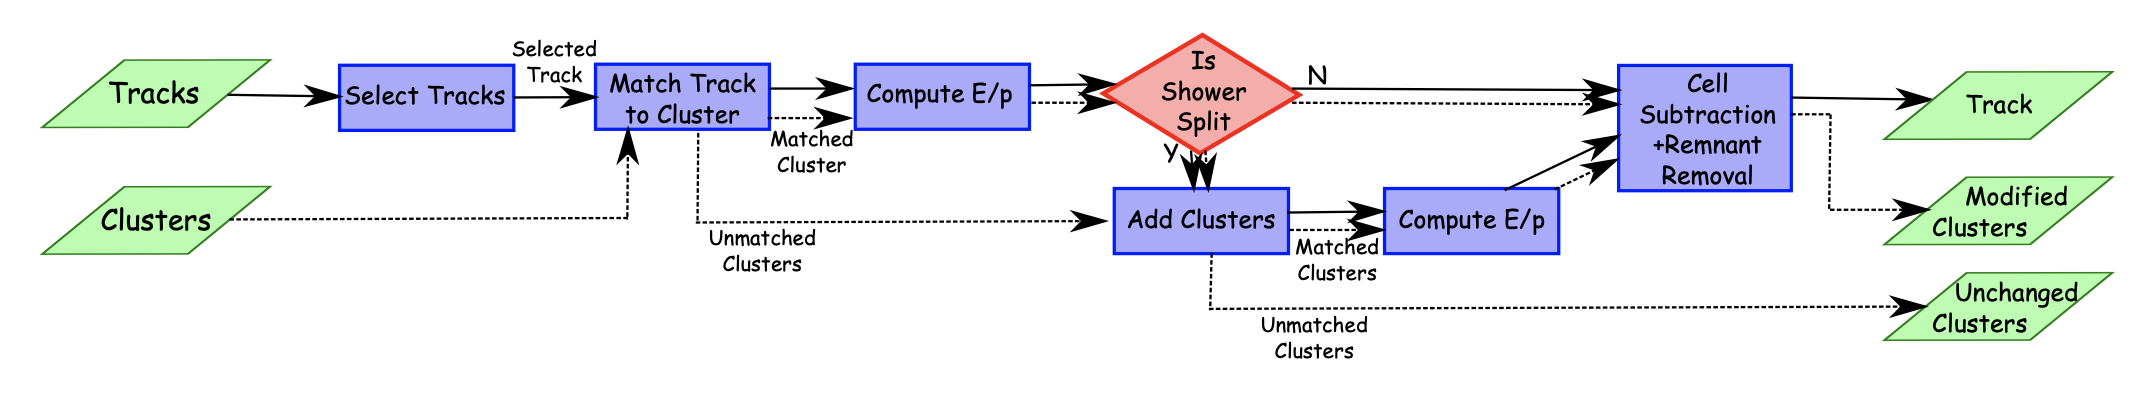
\includegraphics[width=0.98\textwidth]{figures/ch5/pflow_diagram}
	\caption{ A flow chart illustrating the particle flow algorithm progression \cite{pflow}. The solid lines indicate the progression of tracks through the algorithm, while the dotted lines indicate the progression of clusters. The process begins with track selection and continues until the energy associated with the tracks has been removed from the calorimeter. At the end charged particle tracks, unmodified topo-clusters, and the remnants of topo-clusters which have had part of their energy removed remain. }
	\label{fig:pflow_diagram}
\end{figure}

\subsection{Jet Clustering}
\label{sec:jet_cluster}
When a parton decays in the detector, its energy deposits often result in multiple calorimeter clusters. For physics purposes, it is useful to combine clusters that likely resulted from an individual parton decay, in order to reconstruct the parton. The process of grouping topo-clusters which were produced by the same parton decay is \textit{jet clustering}. \par

The anti-$k_t$ algorithm \cite{anti_kt} as provided by the FastJet library \cite{fast_jet} is most commonly used for jet clustering in the ATLAS experiment, with varying reconstruction radius settings. The anti-$k_t$ algorithm is based on sequential recombination algorithms \cite{seq_comb_alg}. A sequential recombination considers the distance $d_{ij}$ between objects $i$ and $j$ (particles or pseudojets), and the distance $d_{iB}$ between an object $i$ and the beam line $B$. If $d_{ij}$ between two objects is the smallest distance among those considered, $i$ and $j$ are combined into a pseudojet. The process continues until the smallest distance is $d_{iB}$ at which point the object $i$ is determined to be a jet and removed from the objects in consideration. The procedure is repeated with the remaining objects until there are none remaining \cite{anti_kt}. \par

The anti-$k_t$ algorithm adopts this procedure, but modifies the distance measurements $d_{ij}$ and $d_{iB}$ to consider the transverse momentum $k_t$:

\begin{subequations}
       	\begin{align}
		d_{ij} &= \min{(k_{ti}^{2p},k_{tj}^{2p})}\frac{\Delta_{ij}^{2}}{R^2}, \\
		d_{iB} &= k_{ti}^{2p} .
	\end{align}
\end{subequations}

The addition of the term $p$ allows adjustments to algorithm which govern the relative power of the momentum versus the geometrical scale $\Delta_{i,j}$, which is defined as $\Delta_{i,j} = (y_i - y_j)^2 + (\phi_i - \phi_j)^2$ where $y_i$ and $\phi_i$ are respectively the rapidity and azimuth of particle $i$ \cite{anti_kt}. The radius parameter $R$ is chosen and determines the geometric cone size \cite{seq_comb_alg}. \par

In the case $p=1$ the inclusive $k_t$ algorithm \cite{seq_comb_alg} is recovered, which is a standard sequential combination jet clustering algorithm. In the case $p=0$, the Cambridge/Aachen sequential combination algorithm \cite{aachen} is recovered. The case $p=-1$ gives rise to the anti-$k_t$ algorithm. The impact of this choice means that the distance $d_{ij}$ between many soft particles is larger than between soft and hard particles. Therefore, soft particles tend to cluster with hard ones before they cluster with other soft particles. They key feature of this behavior is that soft particles do not modify the shape of the jets. This leads to the creation of circular conical jets, a desirable feature which sequential combination algorithms and cone algorithms struggle to achieve. Figure~\ref{fig:jet_algorithms} compares anti-$k_t$ jet formation with the inclusive $k_t$ and Cambridge/Aachen algorithms mentioned here, as well as the SIScone algorithm \cite{siscone}, which checks for sets of stable cones compatible with the observed radiation. \par

\begin{figure}[h]
        \centering
	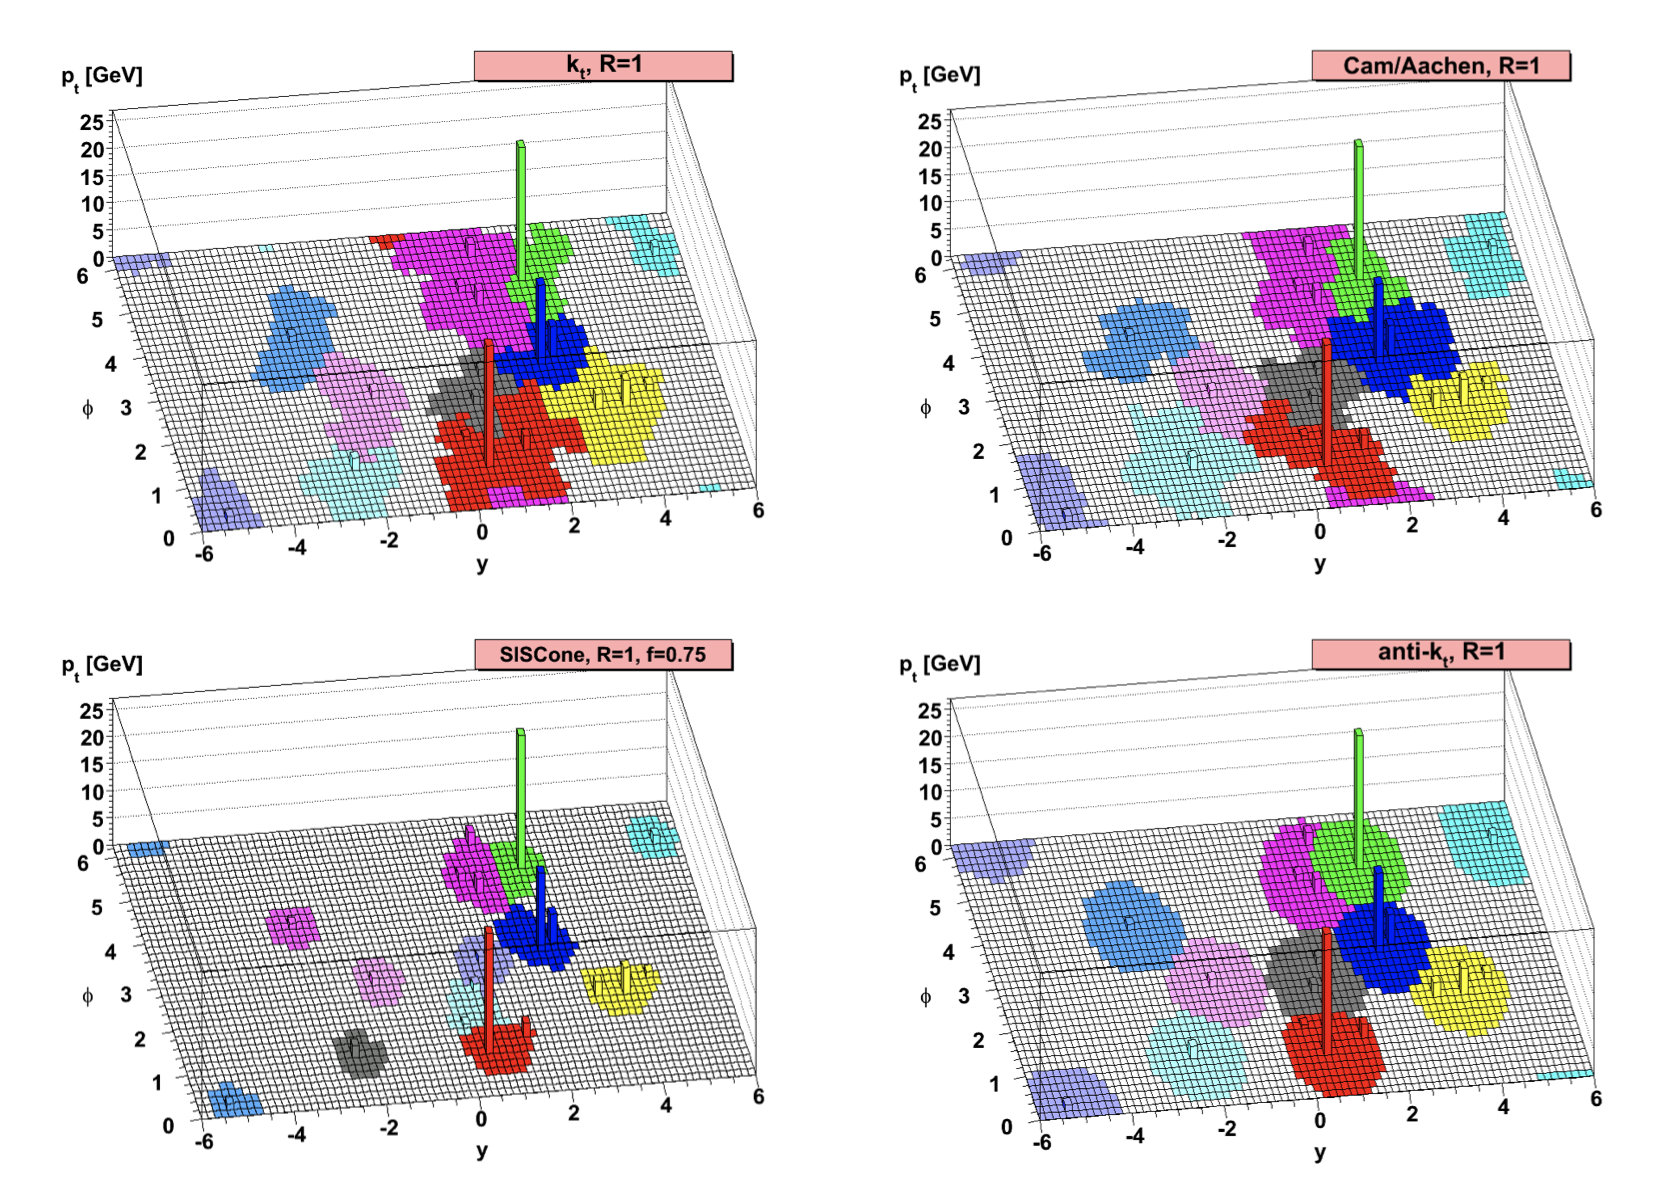
\includegraphics[width=0.9\textwidth]{figures/ch5/jet_algorithms}
	\caption{ A comparison of jet clustering with four different jet algorithms. The anti-$k_t$ algorithm is observed to create the most conical jets, where the shape of the jet is immune to the presence of soft radiation \cite{anti_kt}. }
	\label{fig:jet_algorithms}
\end{figure}

Any useful jet clustering algorithm must satisfy the requirements of infrared safety and collinear (IRC) safety. Infrared safety implies that the resulting set of jets is unaltered by the presence of additional soft particles in the list of seed clusters. As explained above, the anti-$k_t$ algorithm is naturally infrared safe. Collinear safety requires that the final set of jets is not impacted by collinear splitting of one of the jets. If the hardest particle $p_1$ is split into a collinear pair $(p_{1a},p_{1b})$ (as is common in the fragmentation process for a hard parton), the jet clustering algorithm must still recognize $(p_{1a},p_{1b})$ as the hardest jet in the collision. If another softer particle $p_2$ with $p_{t,1a},p_{t,1b} < p_{t,2} < p_{t,1}$ is instead considered the hardest particle in the event, a different final set of jets would be returned. Collinear safety is a requirement of perturbative QCD, to ensure non-divergent higher-order calculations \cite{collinear_safety}. The anti-$k_t$ algorithm's tendency to cluster hard particles first ensures its collinear safety. By satisfying the IRC safety requirement, anti-$k_t$ jets can be calculated using perturbative QCD, which improves comparisons with theory. 
 
\subsection{Ghost Track Association}
\label{sec:ghost}
Once a collection of jets has been created, the jet objects can be studied at both the event-level and the jet-level. In the event-level picture, the momentum, energy, and geometric orientation of the jets within an event are considered. This yields important information about decay of any resonant heavy objects, the total energy in the event, and the distribution of energy amongst the jets. In the jet-level picture, the particle constituents of the jet are considered. The momentum, energy, and geometric orientation of the associated particle tracks provides a low-level picture of the jet, which can help determine if the properties of the jet are consistent with standard QCD, or if new physics processes might be represented within the low-level patterns. Jet-level analysis is also widely used in flavor tagging. \par

For anti-$k_t$ jets with a radius parameter $R=0.4$, one way of studying the jet-level picture is through considering the ghost-associated tracks. Track association is the process of determining which tracks should be considered associated with a given jet. In the ghost association algorithm, the anti-$k_t$ clustering algorithm is used for the collection of tracks and calorimeter clusters \cite{ghosts2}. However, the tracks are considered to have infinitesimal momentum (\textit{ghosts}), so their addition to a jet object does not alter the four-momentum of the jet. This ensures the final jet collection is not altered by the presence of the ghost tracks in the reclustering, but information about the associated tracks for each reconstructed jet becomes available \cite{ghosts1}. \par

Ghost tracks are of particular importance to this analysis, as a means of providing a low-level picture of the shape of $R=0.4$ jets, and discriminating Standard Model QCD-like jets from dark QCD-like jets. 

\section{Missing Transverse Energy}
A simple principle leveraged in ATLAS physics analyses is checking for conservation of momentum among the products of any $pp$ collisions. The initial state transverse momentum of any $pp$ collision is always zero, so the transverse momentum of all final state particles should likewise be zero. The missing transverse energy, \met~, is determined by the magnitude of the negative momentum vector sum of all final state objects resulting from the $pp$ collision. \par

Specifically, the objects considered in the \met~calculation are photons, electrons, muons, jets, and soft terms. The first four items comprise the hard components of the \met~calculation, and have been discussed previously in this chapter. The final item represents a collection of \textit{soft terms}, comprising any detector signals not associated to hard detector objects. These can be based on unassociated tracks, or unassociated soft calorimeter clusters. Both are generally not used in the same calculation to avoid double counting of soft terms. In this analysis the calorimeter cluster soft terms are considered in the \met~calculation. \par

\met~can arise due to non-interacting Standard Model objects such as a neutrinos, fake sources such as mis-reconstructed objects and dead detector regions, or in some theories, non-interacting BSM objects such as a dark matter candidate particles. To understand the amount of \met~attributable to detector noise and mis-reconstruction, \met~is studied in $Z\rightarrow \mu\mu$ where little real \met~is expected \cite{met_res}. As Figure~\ref{fig:met_res} illustrates, the resolution of \met~generally decreases as \met~increases, due to detector resolution effects. As \met~is an important quantity for most dark QCD analyses, limitations in the accuracy of the \met~calculation must be considered.

\begin{figure}[h]
        \centering
	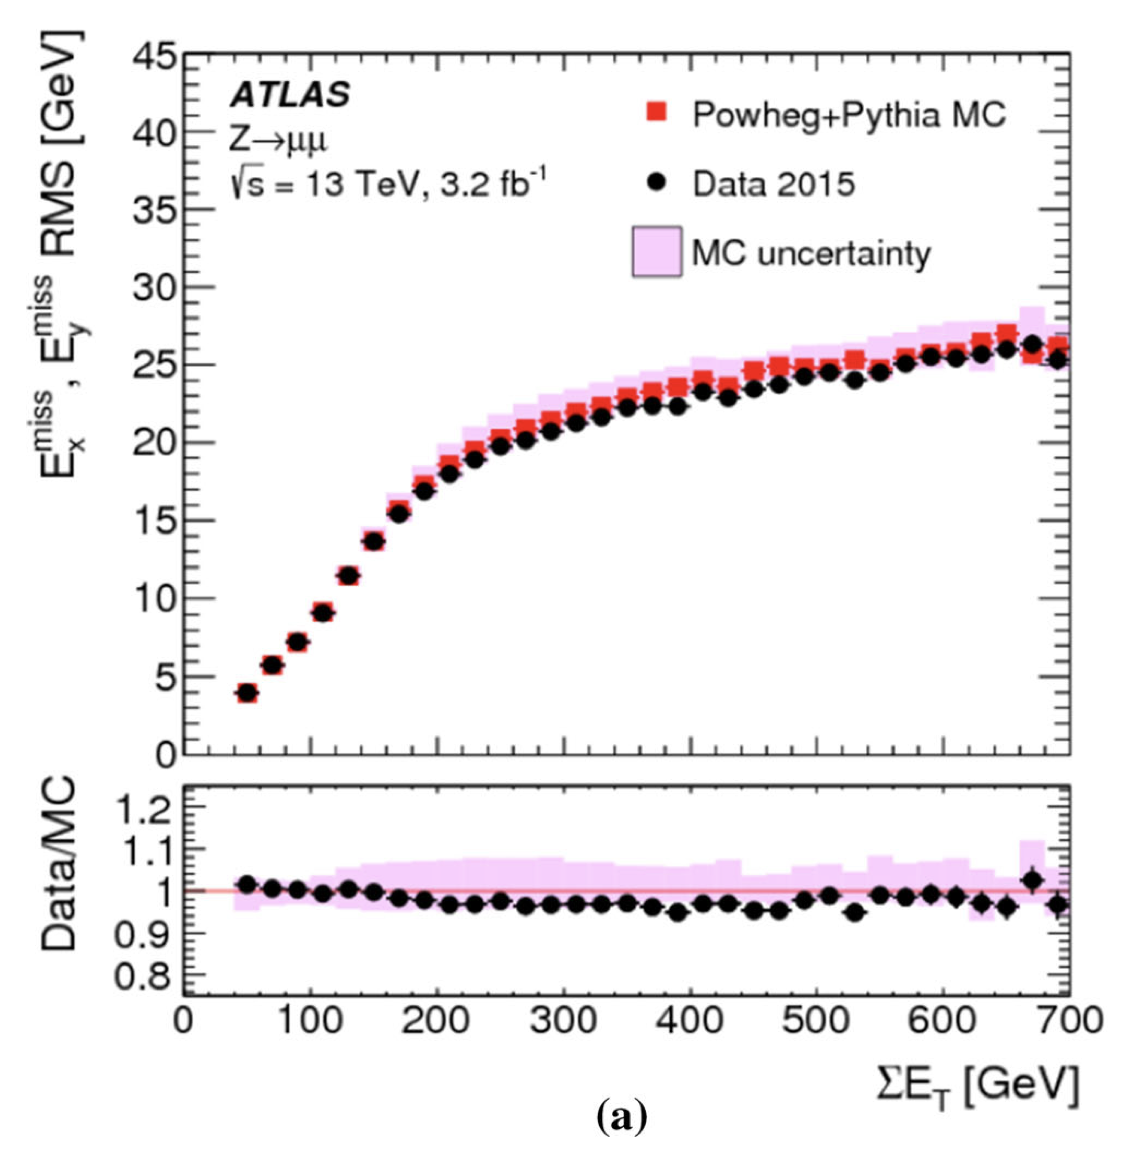
\includegraphics[width=0.45\textwidth]{figures/ch5/met_res}
	\caption{ A comparison of MC simulation and data for $Z\rightarrow\mu\mu$ events where real \met~= 0 \cite{met_res}. The resolution of the missing energy in the transverse $(x-y)$ plane is observed to increase with increasing total $\sum E_T$. }
	\label{fig:met_res}
\end{figure}
